\definecolor{c7}{RGB}{255, 197, 0}
\definecolor{c8}{RGB}{178,204,227}
\definecolor{c9}{RGB}{255, 0, 255}
\vspace{2.5cm}
\hspace{0.5cm}
% GNUPLOT: LaTeX picture with Postscript
\begingroup
  \makeatletter
  \providecommand\color[2][]{%
    \GenericError{(gnuplot) \space\space\space\@spaces}{%
      Package color not loaded in conjunction with
      terminal option `colourtext'%
    }{See the gnuplot documentation for explanation.%
    }{Either use 'blacktext' in gnuplot or load the package
      color.sty in LaTeX.}%
    \renewcommand\color[2][]{}%
  }%
  \providecommand\includegraphics[2][]{%
    \GenericError{(gnuplot) \space\space\space\@spaces}{%
      Package graphicx or graphics not loaded%
    }{See the gnuplot documentation for explanation.%
    }{The gnuplot epslatex terminal needs graphicx.sty or graphics.sty.}%
    \renewcommand\includegraphics[2][]{}%
  }%
  \providecommand\rotatebox[2]{#2}%
  \@ifundefined{ifGPcolor}{%
    \newif\ifGPcolor
    \GPcolorfalse
  }{}%
  \@ifundefined{ifGPblacktext}{%
    \newif\ifGPblacktext
    \GPblacktexttrue
  }{}%
  % define a \g@addto@macro without @ in the name:
  \let\gplgaddtomacro\g@addto@macro
  % define empty templates for all commands taking text:
  \gdef\gplfronttext{}%
  \gdef\gplfronttext{}%
  \makeatother
  \ifGPblacktext
    % no textcolor at all
    \def\colorrgb#1{}%
    \def\colorgray#1{}%
  \else
    % gray or color?
    \ifGPcolor
      \def\colorrgb#1{\color[rgb]{#1}}%
      \def\colorgray#1{\color[gray]{#1}}%
      \expandafter\def\csname LTw\endcsname{\color{white}}%
      \expandafter\def\csname LTb\endcsname{\color{black}}%
      \expandafter\def\csname LTa\endcsname{\color{black}}%
      \expandafter\def\csname LT0\endcsname{\color[rgb]{1,0,0}}%
      \expandafter\def\csname LT1\endcsname{\color[rgb]{0,1,0}}%
      \expandafter\def\csname LT2\endcsname{\color[rgb]{0,0,1}}%
      \expandafter\def\csname LT3\endcsname{\color[rgb]{1,0,1}}%
      \expandafter\def\csname LT4\endcsname{\color[rgb]{0,1,1}}%
      \expandafter\def\csname LT5\endcsname{\color[rgb]{1,1,0}}%
      \expandafter\def\csname LT6\endcsname{\color[rgb]{0,0,0}}%
      \expandafter\def\csname LT7\endcsname{\color[rgb]{1,0.3,0}}%
      \expandafter\def\csname LT8\endcsname{\color[rgb]{0.5,0.5,0.5}}%
    \else
      % gray
      \def\colorrgb#1{\color{black}}%
      \def\colorgray#1{\color[gray]{#1}}%
      \expandafter\def\csname LTw\endcsname{\color{white}}%
      \expandafter\def\csname LTb\endcsname{\color{black}}%
      \expandafter\def\csname LTa\endcsname{\color{black}}%
      \expandafter\def\csname LT0\endcsname{\color{black}}%
      \expandafter\def\csname LT1\endcsname{\color{black}}%
      \expandafter\def\csname LT2\endcsname{\color{black}}%
      \expandafter\def\csname LT3\endcsname{\color{black}}%
      \expandafter\def\csname LT4\endcsname{\color{black}}%
      \expandafter\def\csname LT5\endcsname{\color{black}}%
      \expandafter\def\csname LT6\endcsname{\color{black}}%
      \expandafter\def\csname LT7\endcsname{\color{black}}%
      \expandafter\def\csname LT8\endcsname{\color{black}}%
    \fi
  \fi
    \setlength{\unitlength}{0.0300bp}%
    \ifx\gptboxheight\undefined%
      \newlength{\gptboxheight}%
      \newlength{\gptboxwidth}%
      \newsavebox{\gptboxtext}%
    \fi%
    \setlength{\fboxrule}{0.5pt}%
    \setlength{\fboxsep}{1pt}%
\begin{picture}(8000.00,6000.00)%
    \gplgaddtomacro\gplfronttext{%
%      \colorrgb{0.15,0.15,0.15}%
      %\put(-52,4522){\makebox(0,0)[r]{\strut{}\small $1$$ \cdot $$10\texttt{e}$$+$$2$}}%
      %\colorrgb{0.15,0.15,0.15}%
      %\put(-52,4940){\makebox(0,0)[r]{\strut{}\small $2 $$\cdot $$10\texttt{e}$$+$$2$}}%
      %\colorrgb{0.15,0.15,0.15}%
      %\put(-52,5184){\makebox(0,0)[r]{\strut{}\small $3 $$\cdot $$10\texttt{e}$$+$$2$}}%
      %\colorrgb{0.15,0.15,0.15}%
      %\put(-52,5358){\makebox(0,0)[r]{\strut{}\small $4 $$\cdot $$10\texttt{e}$$+$$2$}}%
      %\colorrgb{0.15,0.15,0.15}%
      %%\put(-52,5775){\makebox(0,0)[r]{\strut{}\small $8 $$\cdot $$10\texttt{e}$$+$$2$}}%
      %\colorrgb{0.15,0.15,0.15}%
      %\put(-52,5910){\makebox(0,0)[r]{\strut{}\small $10 $$\cdot $$10\texttt{e}$$+$$2$}}%
      %\colorrgb{0.15,0.15,0.15}%
      %\put(468,4239){\makebox(0,0){\strut{}}}%
      %\colorrgb{0.15,0.15,0.15}%
      %\put(1244,4239){\makebox(0,0){\strut{}}}%
      %\colorrgb{0.15,0.15,0.15}%
      %\put(2020,4239){\makebox(0,0){\strut{}}}%
      %\colorrgb{0.15,0.15,0.15}%
      %\put(2795,4239){\makebox(0,0){\strut{}}}%
      %\colorrgb{0.15,0.15,0.15}%
      %\put(3571,4239){\makebox(0,0){\strut{}}}%
    }%
    \gplgaddtomacro\gplfronttext{%
      \colorrgb{0.00,0.00,0.00}%
      %\put(3999,6159){\makebox(0,0){\strut{}Κατανομές αριθμού σαρώσεων χάρτη}}%
      \put(2019,4459){\makebox(0,0){\strut{}\footnotesize $\sigma_{\bm{M}} = 0.0$ m}}%
      \put(6019,4459){\makebox(0,0){\strut{}\footnotesize $\sigma_{\bm{M}} = 0.05$ m}}%
      \put(2999,4959){\makebox(0,0){\strut{}{\color{c7}{\rule[0.6mm]{0.5cm}{0.5mm}}}\small \texttt{x1}}}
      \put(3999,4959){\makebox(0,0){\strut{}{\color{c8}{\rule[0.6mm]{0.5cm}{0.5mm}}}\small \texttt{uf}}}
      \put(4999,4959){\makebox(0,0){\strut{}{\color{c9}{\rule[0.6mm]{0.5cm}{0.5mm}}}\small \texttt{fm}}}
    }%
    \gplgaddtomacro\gplfronttext{%
      \colorrgb{0.15,0.15,0.15}%
      \put(3908,4522){\makebox(0,0)[r]{\strut{}}}%
      \colorrgb{0.15,0.15,0.15}%
      \put(3908,4940){\makebox(0,0)[r]{\strut{}}}%
      \colorrgb{0.15,0.15,0.15}%
      \put(3908,5184){\makebox(0,0)[r]{\strut{}}}%
      \colorrgb{0.15,0.15,0.15}%
      \put(3908,5358){\makebox(0,0)[r]{\strut{}}}%
      \colorrgb{0.15,0.15,0.15}%
      \put(3908,5775){\makebox(0,0)[r]{\strut{}}}%
      \colorrgb{0.15,0.15,0.15}%
      \put(3908,5910){\makebox(0,0)[r]{\strut{}}}%
      \colorrgb{0.15,0.15,0.15}%
      \put(4428,4239){\makebox(0,0){\strut{}}}%
      \colorrgb{0.15,0.15,0.15}%
      \put(5204,4239){\makebox(0,0){\strut{}}}%
      \colorrgb{0.15,0.15,0.15}%
      \put(5980,4239){\makebox(0,0){\strut{}}}%
      \colorrgb{0.15,0.15,0.15}%
      \put(6755,4239){\makebox(0,0){\strut{}}}%
      \colorrgb{0.15,0.15,0.15}%
      \put(7531,4239){\makebox(0,0){\strut{}}}%
    }%
    \gplgaddtomacro\gplfronttext{%
    }%
    \gplgaddtomacro\gplfronttext{%
      \colorrgb{0.15,0.15,0.15}%
      \put(-52,2260){\makebox(0,0)[r]{\strut{}\small $0.0$}}%
      \colorrgb{0.15,0.15,0.15}%
      \put(-52,2683){\makebox(0,0)[r]{\strut{}\small $0.100$}}%
      \colorrgb{0.15,0.15,0.15}%
      \put(-52,3105){\makebox(0,0)[r]{\strut{}\small $0.200$}}%
      \colorrgb{0.15,0.15,0.15}%
      \put(-52,3528){\makebox(0,0)[r]{\strut{}\small $0.300$}}%
      \colorrgb{0.15,0.15,0.15}%
      \put(468,2040){\makebox(0,0){\strut{}}}%
      \colorrgb{0.15,0.15,0.15}%
      \put(1244,2040){\makebox(0,0){\strut{}}}%
      \colorrgb{0.15,0.15,0.15}%
      \put(2020,2040){\makebox(0,0){\strut{}}}%
      \colorrgb{0.15,0.15,0.15}%
      \put(2795,2040){\makebox(0,0){\strut{}}}%
      \colorrgb{0.15,0.15,0.15}%
      \put(3571,2040){\makebox(0,0){\strut{}}}%
    }%
    \gplgaddtomacro\gplfronttext{%
      \colorrgb{0.00,0.00,0.00}%
      \put(3999,3959){\makebox(0,0){\strut{}\footnotesize  Κατανομές ολικού χρόνου εκτέλεσης [sec]}}%
    }%
    \gplgaddtomacro\gplfronttext{%
      \colorrgb{0.15,0.15,0.15}%
      \put(3908,2260){\makebox(0,0)[r]{\strut{}}}%
      \colorrgb{0.15,0.15,0.15}%
      \put(3908,2683){\makebox(0,0)[r]{\strut{}}}%
      \colorrgb{0.15,0.15,0.15}%
      \put(3908,3105){\makebox(0,0)[r]{\strut{}}}%
      \colorrgb{0.15,0.15,0.15}%
      \put(3908,3528){\makebox(0,0)[r]{\strut{}}}%
      \colorrgb{0.15,0.15,0.15}%
      \put(4428,2040){\makebox(0,0){\strut{}}}%
      \colorrgb{0.15,0.15,0.15}%
      \put(5204,2040){\makebox(0,0){\strut{}}}%
      \colorrgb{0.15,0.15,0.15}%
      \put(5980,2040){\makebox(0,0){\strut{}}}%
      \colorrgb{0.15,0.15,0.15}%
      \put(6755,2040){\makebox(0,0){\strut{}}}%
      \colorrgb{0.15,0.15,0.15}%
      \put(7531,2040){\makebox(0,0){\strut{}}}%
    }%
    \gplgaddtomacro\gplfronttext{%
    }%
    \gplgaddtomacro\gplfronttext{%
      \colorrgb{0.15,0.15,0.15}%
      \put(-52,60){\makebox(0,0)[r]{\strut{}\small $0.0$}}%
      \colorrgb{0.15,0.15,0.15}%
      \put(-52,483){\makebox(0,0)[r]{\strut{}\small $0.050$}}%
      \colorrgb{0.15,0.15,0.15}%
      \put(-52,905){\makebox(0,0)[r]{\strut{}\small $0.100$}}%
      \colorrgb{0.15,0.15,0.15}%
      \put(-52,1328){\makebox(0,0)[r]{\strut{}\small $0.150$}}%
      \colorrgb{0.15,0.15,0.15}%
      \put(468,-160){\makebox(0,0){\strut{}\footnotesize $0.01$}}%
      \colorrgb{0.15,0.15,0.15}%
      \put(1244,-160){\makebox(0,0){\strut{}\footnotesize $0.03$}}%
      \colorrgb{0.15,0.15,0.15}%
      \put(2020,-160){\makebox(0,0){\strut{}\footnotesize $0.05$}}%
      \colorrgb{0.15,0.15,0.15}%
      \put(2795,-160){\makebox(0,0){\strut{}\footnotesize $0.10$}}%
      \colorrgb{0.15,0.15,0.15}%
      \put(3571,-160){\makebox(0,0){\strut{}\footnotesize $0.20$}}%
    }%
    \gplgaddtomacro\gplfronttext{%
      \colorrgb{0.15,0.15,0.15}%
      \put(3999,-790){\makebox(0,0){\strut{}\footnotesize Τυπική απόκλιση διαταραχών $\sigma_R$ [m]}}%
      \colorrgb{0.00,0.00,0.00}%
      \put(3999,1759){\makebox(0,0){\strut{}\footnotesize  Κατανομές ολικού χρόνου εκτέλεσης (Αναγωγή σε αναπαράσταση χάρτη μέσω πλέγματος $[1]$) [sec]}}%
    }%
    \gplgaddtomacro\gplfronttext{%
      \colorrgb{0.15,0.15,0.15}%
      \put(3908,60){\makebox(0,0)[r]{\strut{}}}%
      \colorrgb{0.15,0.15,0.15}%
      \put(3908,483){\makebox(0,0)[r]{\strut{}}}%
      \colorrgb{0.15,0.15,0.15}%
      \put(3908,905){\makebox(0,0)[r]{\strut{}}}%
      \colorrgb{0.15,0.15,0.15}%
      \put(3908,1328){\makebox(0,0)[r]{\strut{}}}%
      \colorrgb{0.15,0.15,0.15}%
      \put(4428,-160){\makebox(0,0){\strut{}\footnotesize $0.01$}}%
      \colorrgb{0.15,0.15,0.15}%
      \put(5204,-160){\makebox(0,0){\strut{}\footnotesize $0.03$}}%
      \colorrgb{0.15,0.15,0.15}%
      \put(5980,-160){\makebox(0,0){\strut{}\footnotesize $0.05$}}%
      \colorrgb{0.15,0.15,0.15}%
      \put(6755,-160){\makebox(0,0){\strut{}\footnotesize $0.10$}}%
      \colorrgb{0.15,0.15,0.15}%
      \put(7531,-160){\makebox(0,0){\strut{}\footnotesize $0.20$}}%
    }%
    \put(0,0){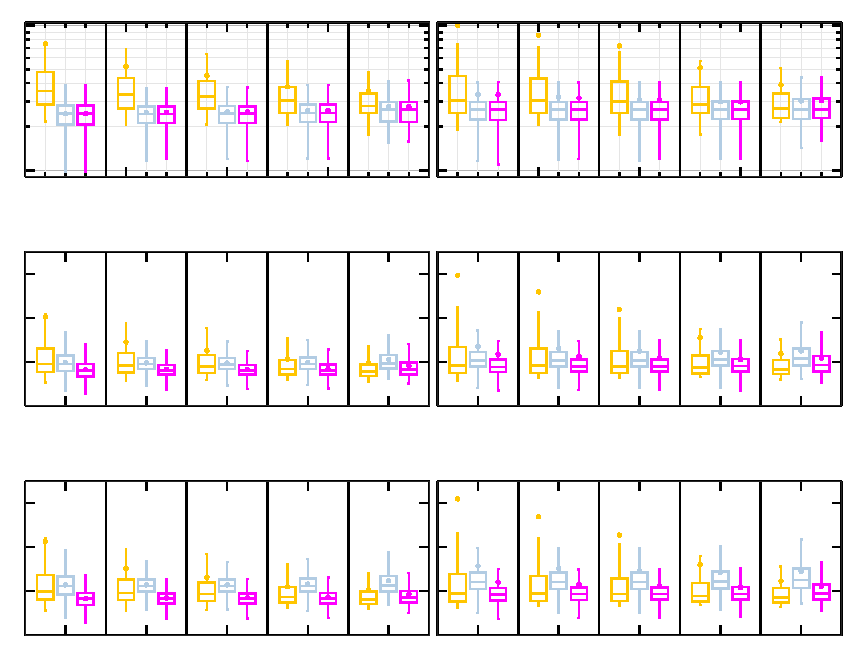
\includegraphics[scale=0.6,clip=true, trim = 0 0 0 100]{./figures/slides/ch6/experiments/boxplots_iterations}}%
    \gplfronttext
  \end{picture}%
\endgroup
